\documentclass{memoir}
\usepackage{hyperref}
\usepackage{graphicx}
\graphicspath{ {figures/} }

\title{Distributed Systems:\\Crossing Intersection with Autonomous Vehicles}

\author{Antonio Toncetti\\Gabriele Venturato\\\\DMIF, University of Udine, Italy}

\date{%Version 0.1, 
	\today}

\begin{document}


%\begin{titlingpage}
\maketitle
\begin{abstract}
The aim of this project is to provide an implemented solution to the problem of autonomous vehicles crossing an intersection.
Although the solution relies on some simplifications, it can be further elaborated to work in a real-case scenario.

The solution proposed in this report is meant to be more general and as modular as possible, in order for it to be possibly extended in a concrete situation.
\end{abstract}
%\end{titlingpage}

\chapter{Introduction}\label{ch:intro}

The problem to solve is the one in which some autonomous vehicles have to cross an intersection without being involved in road accidents. 

The idea is to solve the problem for a generic intersection. The autonomous vehicles can't rely on a central server, they have to cooperate with each other to cross the intersection by taking decisions which ensure a \emph{fair} and \emph{safe} policy. In particular there are two components in the proposed solution: vehicles and the environment. The latter is necessary in this context in order to simulate sensors that are usually inside autonomous vehicles which allows them to interact with the environment (e.g. proximity sensors, GPS, cameras, etc\dots).
The system is \emph{fault tolerant}, but neither byzantine processes nor cybersecurity hazards are taken in consideration, for simplification purpose.

The report starts by analysing the project: Chapter~\ref{ch:analysis} is devoted to functional and non-functional requirements, and system assumptions too. Chapter~\ref{ch:project} contains the description of the general architecture, and specific algorithms.

Following chapters aim to describe details of the implementation, and validation w.r.t. requirements.



\chapter{Analysis}\label{ch:analysis}

This chapter describes in detail some fundamental assumptions about the system, as well as functional and non-functional requirements.

\section{Assumptions}

Some general considerations are here presented. First of all it's assumed a situation in which each autonomous vehicle knows its destination and the roads it is going to travel, since we can assume that each autonomous vehicle has a GPS device on board.

Moreover it's assumed, for sake of simplicity, that all vehicles have the same dimension --- or better: that each vehicle can fit into a single position of the internal model used to represent the roads. Moreover, common physical quantities (like weight, speed, acceleration, etc\dots) are omitted. Instead, the autonomous vehicles move in unit steps governed by the internal model.
\newline

Further assumptions are:

\begin{itemize}
	\item \emph{Faults}: at any moment a failure can arise in vehicles --- software or mechanical. A mechanical failure doesn't compromise the software abilities, but a software failure implies an hardware failure. Since we can assume that if the software fails, the autonomous vehicle stops and goes in ``emergency mode''. It's also assumed that if a crash happens in queues, there's enough space for the other vehicles to overtake the faulty one; but if the crash happens inside the crossroads it must be managed by removing the faulty vehicle with a tow truck (or something similar).
	\item \emph{Moves}: the path that a vehicle can take inside the interception is predefined and known a priori. From each position there's a unique path to each destination, and no one can modify or choose a different path once decided. A visual representation of this assumption can be found in Figure~\ref{fig:intersection-graph}, in which green dots represent positions occupied while crossing, and light-blue dots are the destinations. Once a vehicle reaches its destination, it is considered ``satisfied'', and can not fail anymore, it can only move forward on its own way. Reversing is not allowed.
	\item \emph{Message Delivery}: there exist an upper bound time in message passing between two nodes. This is justified by the fact that all connection are direct, without routers or broker that can cause bottle-necks or network congestion.
\end{itemize}

\begin{figure}
	\centering
	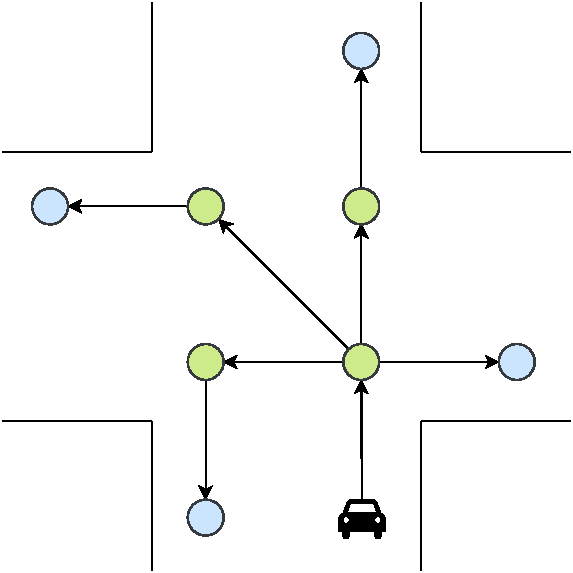
\includegraphics[width=0.4\linewidth]{intersection_graph.pdf}
	\caption{Example of predefined movements that a vehicle can follow in crossing an intersection.}
	\label{fig:intersection-graph}
\end{figure}

\section{Functional requirements}
The solution provides two main modules: \emph{vehicle} and \emph{environment}.

\subsection{Vehicle}
Each vehicle has an internal state at any moment. Moreover he:

\begin{itemize}
	\item knows its position and what happens around, through the environment (in a real context this is handled by sensors like GPS and proximity sensors): it can pick up if there are other vehicles trying to cross, or if there is a vehicle in front or behind it;
	\item communicates with its neighbours by sharing: the direction it wants to travel, its internal state, the next position he is about to reach;
	\item if it's in the queue, it knows nothing other than its internal information and that it is taking part in a queue with someone before and possibly behind, it can communicate only with these two;
	\item if it's in the head of the queue, it can connect with other vehicles (that are the head of other queues) that are crossing the intersection;
\end{itemize}

\subsection{Environment}
The environment represent the vehicle's ability to use its sensors. It knows the intersection shape and dimension; it knows vehicles approaching the crossroads and the ones in the queues; it provides vehicles with all the information they need to safely manoeuvre within the environment.

\section{Non functional requirements}
The system doesn't handle byzantine processes nor cybersecurity issues.

\begin{itemize}
	\item \emph{Safeness}: there can't be more than a vehicle in the same position at the same time;
	\item \emph{Liveness}: if a vehicle approaches the intersection and is waiting to cross it, eventually it will cross it;
	\item \emph{Fairness}: if a vehicle approaches the intersection and is waiting to cross it, there exists a bound to the waiting time;
	\item \emph{Fault Tolerant}: the system is tolerant to hardware and software failures;
	\item \emph{Distributed}: there is no central server, vehicles have to coordinate each other.
\end{itemize}



\chapter{Project}\label{ch:project}
This chapter is devoted to the description of the general architecture, and specific algorithms.

\section{Logical architecture}
The solution leans on two main modules, and a secondary one for tests.

\begin{itemize}
	\item \emph{Vehicle}: it is represented as a finite state automaton. A graphical representation can be seen in Figure~\ref{fig:vehicle-automaton}. Each state represents a situation in which the vehicle can find itself. A vehicle is in Waiting state when it is in the queue and it's not the first. It's in Ready state when it's the first in its queue. It's in Election when an election is needed but the current leader has not yet finished the crossing. Crossing, Crossed, and Crash states are self-explanatory.
	\item \emph{Environment}: it represents the physical environment accessible through autonomous vehicle sensors.
	\item \emph{Random Generator}: it is a module aimed to (pseudo-)randomly generate vehicles that approach the intersection, and it is used to test and validate the solution proposed.
\end{itemize}

\begin{figure}
	\centering
	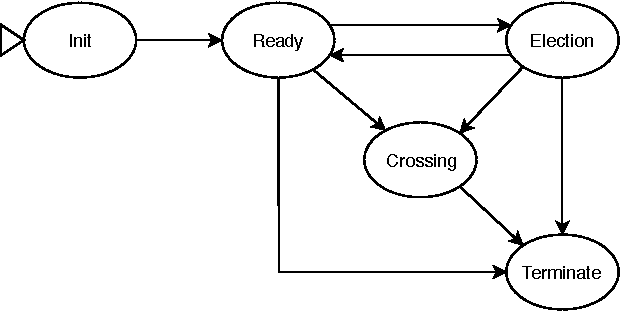
\includegraphics[width=0.8\linewidth]{vehicle_automaton.pdf}
	\caption{Vehicle as a finite state automaton.}
	\label{fig:vehicle-automaton}
\end{figure}

\section{Protocols and algorithms}
This section describes the algorithm to solve the core part of the project. Moreover, some peculiar situation sequence diagrams are presented.

\subsection{Intersection Crossing Algorithm}
Vehicles queue up along the roads leading to an intersection awaiting for their turn to cross. The first vehicle of a queue is the vehicle at the verge of entering the intersection and we will call such vehicle a \emph{participant} of the intersection crossing algorithm.

Note that this algorithm applies to generic intersections. Moreover, it trivially guarantees the \emph{fairness} and \emph{liveness} requirements, thanks to its round robin characteristic.
\\\\
\noindent
The algorithm maintains the following invariant through execution:

\begin{itemize}
	\item one vehicle per time can cross the intersection
	\item only the leader vehicle can cross the intersection
\end{itemize}
Algorithm description:
\begin{enumerate}
	\item The participants (first vehicles in their respective queues) are willing to cross the intersection;
	\item They start a slightly modified version of the Bully Algorithm to elect a leader: it terminates with the leader $L$, and the next leader $L'$, which is the first vehicle after him in a clockwise manner;
	\item $L$ begins to cross the intersection;
	\item After $L$ has successfully crossed the intersection, the participants are informed;
	\item $L'$ identifies the next leader $L''$ by choosing the first vehicle after him in a clockwise manner;
	\item The lead passes to $L'$ informing every participant that it's the new leader;
	\item The algorithm repeats from 3, where $L = L'$ and $L' = L''$.
\end{enumerate}
Additional details:
\begin{itemize}
	\item After the leader election, every participant knows who is the current leader, and who is the next one;
	\item Once the leader starts crossing, the vehicle behind it (if any) becomes a new participant and asks to join the algorithm. Only the leader answers, providing its identity.
	\item Once the vehicle behind the leader move forward, it's assumed that all the vehicles in the queue move forward too.
\end{itemize}
A leader election starts only when new participants don't receive an answer when asking to join the algorithm. In particular: when one or more vehicles join an empty intersection, i.e. when they become participants and no prior participants are available, or when the candidate leader fails before becoming the new leader.

\subsubsection{Managing abnormal cases}

All participants monitor the leader and the candidate leader, if the leader fails, everyone knows who the next leader is (see 2. in the algorithm description).

\begin{itemize}
	\item If the leader fails, the vehicle in clockwise order after him becomes the new leader --- identifying also the next candidate leader --- and the algorithm restarts from 3.
	\item If a (non-crossing) participant fails, the vehicle behind it in the queue becomes immediately a participant, justified by the assumption that in queues there's enough space to overtake the faulty vehicle.
	\item If the leader fails while crossing, a timeout $T$ is needed before it is removed from the intersection. Meanwhile a new election can start, and the new leader can start crossing, but it has to stop if the position in front of him is still occupied from the previous faulty leader.
	\item If the candidate leader fails before becoming the new leader, a new election must be started \emph{after} the current leader have completed the crossing.
\end{itemize}

\subsection{Sequence Diagrams}
This section presents some sequence diagrams of relevant case situations.

\subsubsection{Normal execution of Intersection Crossing Algorithm}
The diagram in Figure~\ref{fig:seq-diag-crossing-intersection} represent the normal execution of the algorithm described above. It starts at the end of the Bully Algorithm, with the $AV_4$ comunication it is the leader and the candidate leader is $AV_1$. It's assumed the queues are enumerated from 1 to 4 in clockwise order.

The leader crosses the intersection by asking the environment if the position in front of it is free, and continues to cross until it reaches its destination.

It's important to note that when the leader starts crossing, the environment notifies $AV_5$ --- which is the one following $AV_4$ in the queue --- that it can move one position forward. Then $AV_5$ is at the verge of the intersection and can communicate with the other participants in order to compete for the crossing.

\begin{figure}
	\centering
	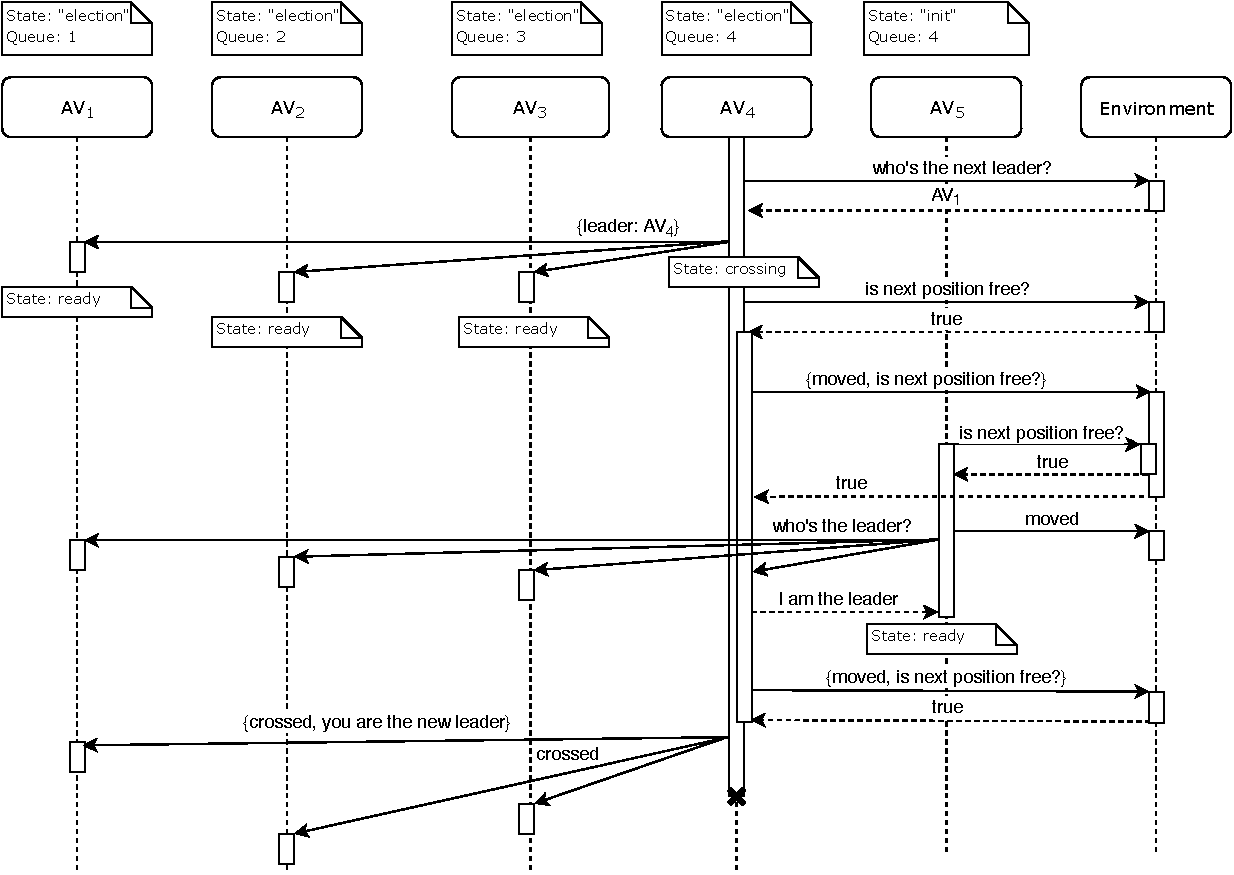
\includegraphics[width=\linewidth]{sequence_diagrams/crossing_intersection.pdf}
	\caption{Sequence diagram on a normal execution of the Intersection Crossing Algorithm described above.}
	\label{fig:seq-diag-crossing-intersection}
\end{figure}

\subsection{Dealing with AV failures}

Leader failures don't cause troubles if they are detected by their relative candidates. Once a candidate detects the failure it automatically ascends to leader and notifies all participants. The normal algorithm flow is restored. The situation is represented by the sequence diagram in Figure~\ref{fig:seq-diag-leader-sw-failure}

\begin{figure}
	\centering
	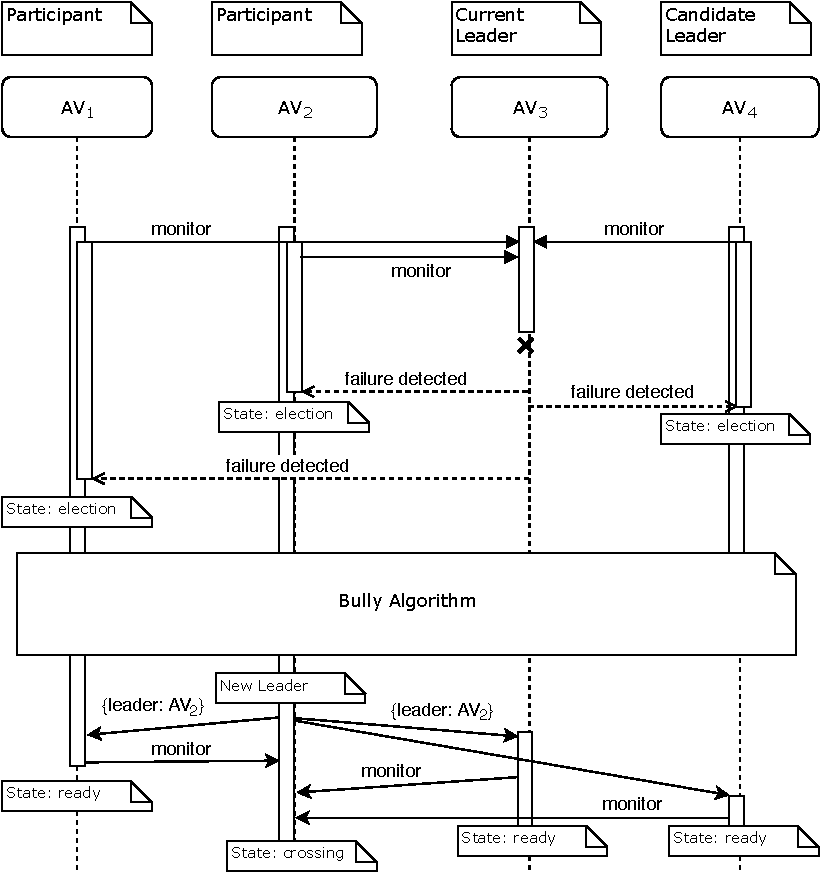
\includegraphics[width=\linewidth]{sequence_diagrams/leader_sw_failure.pdf}
	\caption{Sequence diagram representing a generic leader failure.}
	\label{fig:seq-diag-leader-sw-failure}
\end{figure}


Another delicate situation is the represented in Figure~\ref{fig:seq-diag-new-participant}. The leader fails and before the candidate detects the failure, a new participants asks to join the algorithm. This situation is solved by the assumption that there exist a time bound to message delivery, therefore the new participant knows that in a prefixed amount of time it can receive the message of the new elected leader.

\begin{figure}
	\centering
	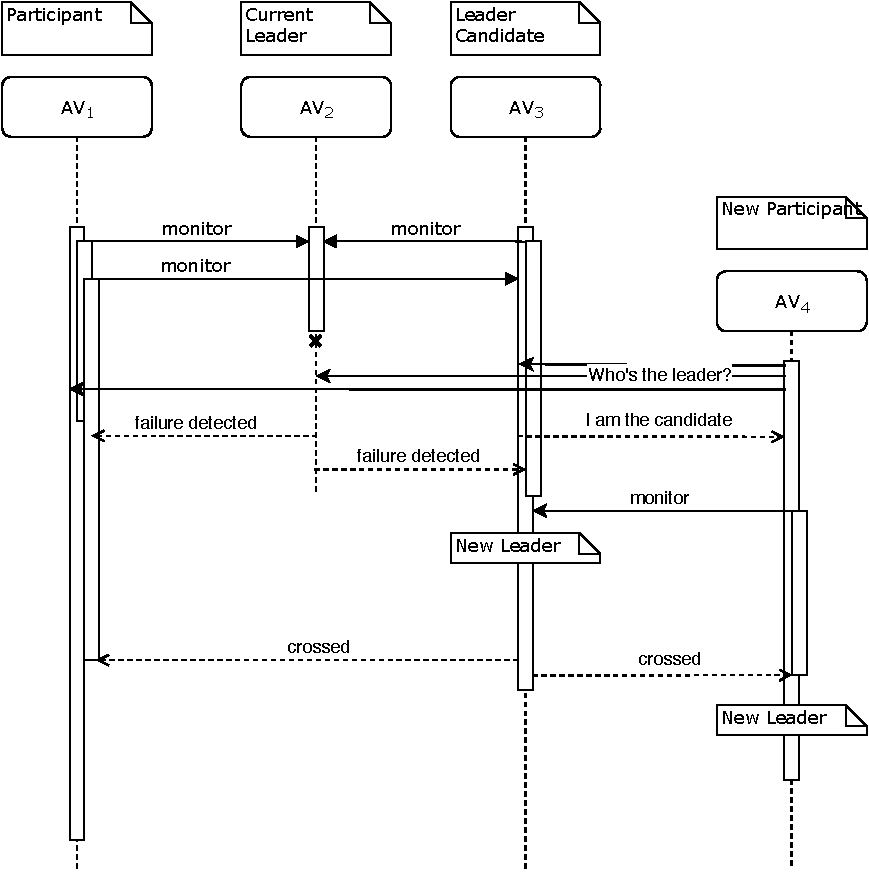
\includegraphics[width=\linewidth]{sequence_diagrams/new_participant.pdf}
	\caption{Sequence diagram of a leader failure happening at the time a new participant joins.}
	\label{fig:seq-diag-new-participant}
\end{figure}

The last situation in Figure~\ref{fig:seq-diag-candidate-failure} represents a failure of the candidate leader. The situation is restored when the leader detects the failure and starts a leader election.

\begin{figure}
	\centering
	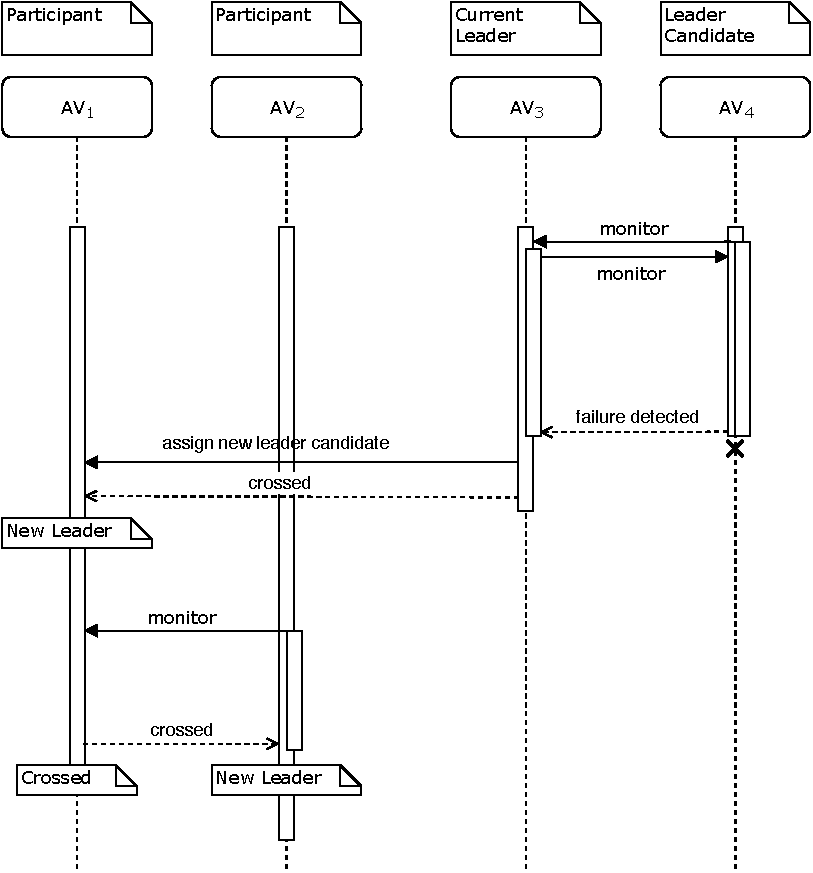
\includegraphics[width=\linewidth]{sequence_diagrams/candidate_failure.pdf}
	\caption{Sequence diagram of a candidate leader failure.}
	\label{fig:seq-diag-candidate-failure}
\end{figure}

\section{Physical architecture and deployment}
The architecture is quite simple, a graphical representation is displayed in Figure~\ref{fig:physical-architecture}. Each Autonomous Vehicle (AV) is a physical node. The Environment represents the world sensed by AVs, so it's not actually a physical node. AVs can ask the environment for information, and they can communicate with their neighbours.

\begin{figure}
	\centering
	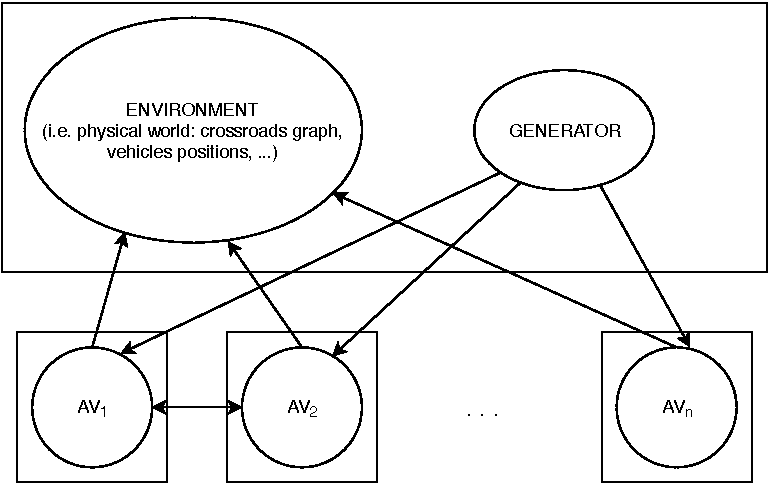
\includegraphics[width=0.8\linewidth]{physical_architecture.pdf}
	\caption{Physical architecture: Environment and Autonomous Vehicles (AV).}
	\label{fig:physical-architecture}
\end{figure}

\section{Development plan}
The proposed solution focuses on a very simplified version of what a real solution could be. In particular the aim is to produce a core solution which satisfies the requirements but that also doesn't contain more than necessary assumptions, and in particular that doesn't rely on non realistic ideas that can lead future development to a blind spot.

If the core simplified part will be easily developed and validated, then some advancement can be pursued, for example:
\begin{itemize}
	\item Add vehicles with priorities, e.g. emergency vehicles;
	\item Dynamically modify paths inside the crossroad if some position becomes unavailable;
	\item Let more than one vehicle per time cross the intersection, maybe with an interface to a planner in order to find the best route (exploiting epistemic planning could be an interesting option).
\end{itemize}


%\chapter{Implementation}
%The project is developed in \href{https://www.erlang.org/}{Erlang}.

%\chapter{Validation}


%\chapter{Conclusions}



%\appendix

%\chapter{Appendix}

\end{document}